\documentclass[a4paper,11pt]{kth-mag}
\usepackage[T1]{fontenc}
\usepackage{textcomp}
\usepackage{lmodern}
\usepackage[latin1]{inputenc}
\usepackage[swedish,english]{babel}
\usepackage{modifications}
\usepackage[backend=bibtex]{biblatex}
% code
\usepackage{listings}
\usepackage{color}

\usepackage{minted}

\usepackage{graphicx}
\pdfoptionpdfminorversion 6

\bibliography{bib/database.bib}

\definecolor{dkgreen}{rgb}{0,0.6,0}
\definecolor{gray}{rgb}{0.5,0.5,0.5}
\definecolor{mauve}{rgb}{0.58,0,0.82}

\lstset{frame=tb,
  language=Java,
  aboveskip=3mm,
  belowskip=3mm,
  showstringspaces=false,
  columns=flexible,
  basicstyle={\small\ttfamily},
  numbers=none,
  keywordstyle=\color{blue},
  commentstyle=\color{dkgreen},
  stringstyle=\color{mauve},
  breaklines=true,
  breakatwhitespace=true
  tabsize=3
}


\title{Lorem ipsum dolor sit amet, sed diam nonummy nibh eui
       mod tincidunt ut laoreet dol}

\subtitle{Duis autem vel eum iruire dolor in hendrerit in
          vulputate velit esse molestie consequat, vel illum
          dolore eu feugiat null}
\foreigntitle{Lorem ipsum dolor sit amet, sed diam nonummy nibh eui
              mod tincidunt ut laoreet dol}
\author{Namn Namnet}
\date{November 2003}
\blurb{Master's Thesis at NADA\\Supervisor: Tjoho\\Examiner: Tjohej}
\trita{TRITA xxx yyyy-nn}
\begin{document}
\frontmatter
\pagestyle{empty}
\removepagenumbers
\maketitle
\selectlanguage{english}

\begin{abstract}
  This is a skeleton for KTH theses. More documentation
  regarding the KTH thesis class file can be found in
  the package documentation.

Lorem ipsum dolor sit amet, consectetuer adipiscing elit. Mauris
purus. Fusce tempor. Nulla facilisi. Sed at turpis. Phasellus eu
ipsum. Nam porttitor laoreet nulla. Phasellus massa massa, auctor
rutrum, vehicula ut, porttitor a, massa. Pellentesque fringilla. Duis
nibh risus, venenatis ac, tempor sed, vestibulum at, tellus. Class
aptent taciti sociosqu ad litora torquent per conubia nostra, per
inceptos hymenaeos.
\end{abstract}

\clearpage

\begin{foreignabstract}{swedish}
  Denna fil ger ett avhandlingsskelett.
  Mer information om \LaTeX-mallen finns i
  dokumentationen till paketet.

Lorem ipsum dolor sit amet, consectetuer adipiscing elit. Maurisd
purus. Fusce tempor. Nulla facilisi. Sed at turpis. Phasellus eu
ipsum. Nam porttitor laoreet nulla. Phasellus massa massa, auctor
rutrum, vehicula ut, porttitor a, massa. Pellentesque fringilla. Duis
nibh risus, venenatis ac, tempor sed, vestibulum at, tellus. Class
aptent taciti sociosqu ad litora torquent per conubia nostra, per
inceptos hymenaeos.
\end{foreignabstract}
\clearpage
\tableofcontents*

\mainmatter
\pagestyle{newchap}

\chapter{Introduction}

\section{Context and system overview}

Data is now at the center of organizations and is increasingly heterogeneous with an explosion of data sources 
that each exposes data in its own format that can be structured, semi-structured or non-structured.
Another major trend is that data processing needs to be real-time, because business men no longer want to wait a whole day 
to have reports and alerts on their business data. Last but not least, the volume of data that enterprises need to analyze is constantly growing, which is commonly referred as "Big Data".
\\

To achieve these requirements, traditional monolithic Data Wharehouse softwares start to be out-dated. They often
propose to deal only with structured data to map it to a relational model, and are often batch-oriented: 
the ETL mechanism (data extraction, transform and load) regularly happens once or twice per day, and there is no mechanism 
for real-time subscriptions on new events happening on the data (as highlighted by Jay Kreps, engineer at LinkedIn, 
in his article "The Log: What every software engineer should know about real-time data's unifying abstraction" \footfullcite{bib:linkedinLog}). Moreover,
Data Integration, Data Storage and Data Reporting are often coupled into a single monolithic software.
\\

Thus, a new kind of architecture for Data Integration and Data Processing is needed in order to meet these new requirements: real-time processing of potentially big volumes of unstructured data. This thesis presents an architecture that solves this problem using \textit{decoupled components} that communicate with \textit{immutable events} that represent data changes. Events flow across the platform enabling components to react to data changes in various ways. Real-time should be understood as \textit{soft} real-time in comparison to batch modes that are more common in Big Data frameworks. For example, event propagation across the platform should be measured in milliseconds or seconds, whereas batch jobs are often measured in hours. Moreover, in a real-time platform, the notion of Big Data is more related to the push rate of events than the size of an event itself. Thus, the platform should take care of possible performance problems in order to handle high push rates.

Each event represents the change (creation, update or deletion) made to a data resource at a particular time. Based on the Event-Sourcing principle \footfullcite{bib:eventSourcing}, events are stored in a Journal that is an ordered sequence of events. Then, the stream of events coming from the Journal can be processed by data consumers that can react to the change of data (see Figure \ref{fig:main_archi} for the global architecture). 
An example of data consumer can be one that maintains a pre-computed view on the data that is updated upon each event, or one that pushes 
notifications to another service upon the reception of some kinds of events.
\\

An example use case is when an organization uses different SaaS services for each of its teams. For instance, the sales
team uses a SaaS software to process their sales pipeline, the project management team uses another SaaS software to manage
the production teams, etc... Without a central data backbone, it is not possible to have a global view on the company data.
The platform I present in this thesis can integrate these different SaaS softwares using their REST API, detect what
changes have been made on the data, and emit the corresponding events. As a result, data consumers can use these events
to update dashboards about the company data in real-time, mixing the data coming from different sources. A data consumer can also push a
notification to SaaS service X when it receives an event from SaaS service Y, allowing real-time synchronization between
heterogeneous services.
\\

An advantage of Event Sourcing is that the whole history of the system is stored. Events are immutable changes made to the data
and are always appended to the Journal (never deleted or modified). As a result, the system stores not only the current state
of the data, but also all its previous states. This allows two interesting properties.

First, it is possible to query past states of the data. This can be very useful for various use cases
where one is interested in the data history, for example a financial audit.

Moreover, storing all the data changes greatly improves the fault-tolerance of the system. As events are not deleted, it is always possible 
to come back in the past in the Journal, delete some delete events that were put by mistake, and replay the events after
them to re-build the system in a right state. This is also referred as Human Fault-Tolerance \footfullcite{bib:human-ft}: in a mutable system,
if an user accidentally delete a data entry, it is lost for ever. But in an immutable system, the deletion is just another
event added to the journal. Figure \ref{fig:event-sourcing} illustrates the difference between a mutable system and an immutable event-sourced system.
\\ 

\begin{figure}[h]
  \begin{center}
    \makebox[\textwidth]{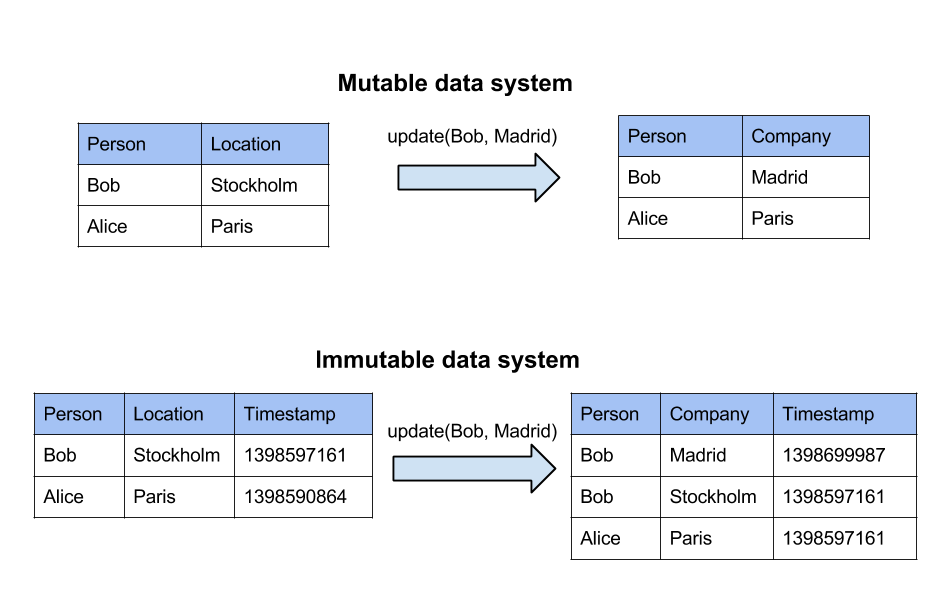
\includegraphics[width=1.0\textwidth]{img/event-sourcing.png}}
    \caption{Immutable datastore and the Event Sourcing principle}
    \label{fig:event-sourcing}
  \end{center}
\end{figure}

This kind of architecture is also known as CQRS \footfullcite{bib:cqrs}. The core principle of CQRS is to decouple the write part and the read part
of a system. The write part (Data Integration) only needs to push immutable events to the Journal in an append-only fashion, which
is very efficient because there is no mutation of the data and no read-write contentions as in traditional databases.
The read part is a set of denormalized pre-computed views that are optimized for low read latency (as the views are automatically re-computed
when a new related event comes in).
An obvious downside of such an architecture is that data is eventually consistent: when a data producer has received the acknowledgment
from the Journal, there is no guarantee that data consumers has already processed the event and updated the data view.

This model also allows very easy distribution of the platform because it enables a message-oriented
architecture where each component (data producer, journal, data consumers with data views) only exchanges messages (events) with each other (share-nothing architecture).
\\

The platform is composed of three main parts: 
\begin{itemize}
  \item Data Integration, that must integrate several data sources in order to emit 
events (data changes) to the Journal. 
  \item Journal, an abstraction for a sequence of immutable events. The Journal must expose methods to insert events,
  and expose methods to subscribe to the stream of events.
  \item Stream processing, where one can define a tree of data consumers (stream processors) that can react to
  events, maintain derived pre-computed views on the data, and emit new streams of events.
\end{itemize}

\begin{figure}[h]
  \begin{center}
    \makebox[\textwidth]{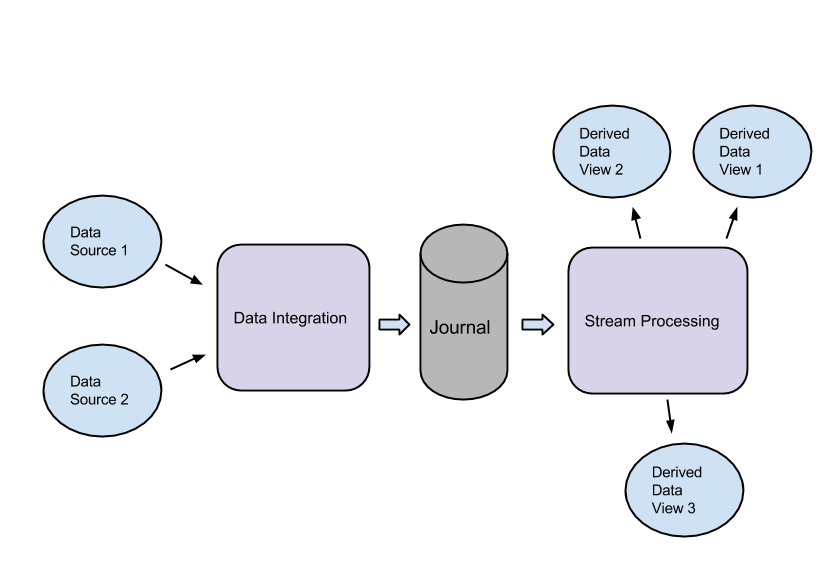
\includegraphics[width=1.0\textwidth]{img/main_archi.png}}
    \caption{Global architecture}
    \label{fig:main_archi}
  \end{center}
\end{figure}

Nonetheless, this kind of evented architecture must be done with a lot of care concerning technical architecture.
The platform needs to do lot of IO in order to push the stream of events from data sources to data consumers, and must
parallelize a lot of operations. Moreover, it must ensure that the stream of events (producers) does not overwhelm the stream
processors (consumers), i.e. if consumers process data slowly, producers must try to slow the push rate. The platform should also deal with possible
failures of components and offer strong guarantees in these cases (like no message loss or duplication).

In order to fulfill those requirements, the platform will apply the principles of the Reactive Manifesto \footfullcite{bib:reactiveManifesto} in order to guarantee
that the platform is \textit{scalable, event-driven, resilient and responsive} (the four Reactive Traits). An asynchronous non-blocking approach with a share-nothing architecture will be used to develop the platform in order to optimize resource consumption, decouple components to be able to distribute them easily, take easily advantage of parallelization and handle failures. 
The platform is developed using functional programming in the Scala programming language \footfullcite{bib:scala} in order to leverage functional programming abstractions to better handle asynchronous and stream-oriented code.
\\


\section{Related works}

There exists several Big Data frameworks for real-time processing. Among them, Apache Kafka \footfullcite{bib:kafka} and Apache Storm \footfullcite{bib:stormframework} have been thoroughly studied for this thesis.
\\

Apache Kafka is a high-throughput distributed messaging system developed at LinkedIn. It is a distributed publish-subscribe system where data producers can send messages in topics and data consumers can subscribe to topics. It is durable by persisting messages on disk and data consumers can pull events with a guaranteed order. However, as it uses a publish-subscribe abstraction, it does not enable the user to define clear stream processing flow structures (such as trees or DAGs) where components are both data consumers (receiving events from parent components) and data producers (sending events to their child components).
\\

Apache Storm is a distributed and fault-tolerant real-time computation framework developed at Twitter. It enables the user to define a DAG of stream processors that can receive event from their parent(s) and send derived events to their children. However, messages are not persisted on disk, so there is no durability, which implies that slow processors are forced to keep past events in-memory if we want fast processors to move on to next events without waiting for slow processors (more details will be given on these types of recurrent stream processing issues in chapter \ref{chapt:streamproc}).
\\

As explained in more details in the thesis, our platform will take some architecture patterns of these two frameworks to achieve an original architecture with a list of properties that none of these frameworks fully provide on their own.

\section{Contributions}

The main contributions of this thesis are:
\begin{itemize}
  \item Definition of the architecture of the Data Integration part and its implementation
  \item Definition of the architecture of the Event Stream Processing part and its implementation as a generic library
  \item Implementation of a business use case application using the generic library for event stream processing, as well as performance tests on this application
\end{itemize}





\chapter{Requirements}

\section{Functional requirements}

This section details the following functional requirements:
\begin{itemize}
  \item Incremental pull of data changes from various data sources' REST APIs with data cleaning and validation.
  \item Insertion of data events in the Journal, ensuring no event duplication and no event loss even in cases of transient failures.
  \item Stream processing system composed of stream processors forming a tree structure. Each processor must ensure an exactly-once semantic for side-effects even in cases of transient failures. The stream processing system must also ensure no event duplication and no event loss even in case of transient failures, which implies a possibility for processors to \textit{replay} the stream.
\end{itemize}

\subsection{Data Integration}

The Data Integration part of the platform needs to integrate several data sources in order to push data events into the Journal. Integration means that it must be able 
to detect the changes made to the data, and push events that can be either create event or update event or delete event.
In the following, we call a data entry a \textit{resource}. A resource is a keyed data defined by its id (for example \verb|/client/1| for a
resource of type client of id 1). Each type of resource has a defined set of fields (for example a client
will have a field name, address, ...).
\\

More specifically, the platform needs to integrate several data sources that expose REST APIs. Such APIs expose information
concerning business data such as new sales information, new financial information...
Each time that a resource is modified in one of these data sources, the platform should detect this change, apply some data cleaning and transformation, create an 
event from it and push it into the Journal.

The problem with most REST APIs is that they are not evented, i.e. they are pulled-based and not pushed-based. 
One must sent an HTTP request to query new data each time they need to. There exists some techniques to stream data via HTTP 1.1 and the 
Chunked Transfer Encoding, but the REST APIs that the platform needs to integrate do not expose such stream interface. 
Thus, the architecture of this part needs to provide a way to perform incremental pull from data sources, and then transform
it in a push stream of events towards the Journal. Moreover, the platform needs to make sure to insert the events in the same
order that they happened in their data source.


\subsection{Journal and Stream Processing}

The Journal must provide a way for data producers to push one or several events that represent the creation, update or 
delete of a resource. Moreover, it must allow data consumers to subscribe to the stream of inserted events. Events must be
immutable and are stored in a sequence that respects the insertion order. The stream of events pushed to the data consumers
(stream processors) must be in the same order than the insertion order and with no event loss or duplication. Of course, the Journal must be persistent to
be able to recover its data after a shutdown or a crash.
\\

The Stream Processing part is the most complex part of the platform. This part should be a library that allows the user
to define a tree a stream processors (see Figure \ref{fig:tree}), where the root of the tree is the Journal. 

\begin{figure}[h]
  \begin{center} 
    \makebox[\textwidth]{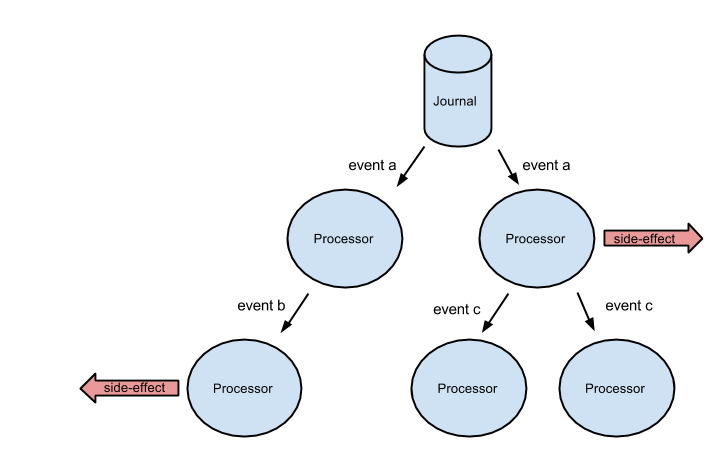
\includegraphics[width=1.0\textwidth]{img/tree.png}}
    \caption{A tree of stream processors}
    \label{fig:tree}
  \end{center}
\end{figure}

A stream processor receives events coming from its parent node. Upon the reception of an event, it can do one or several of these
actions (see Figure \ref{fig:streamprocessor}):
\begin{itemize}
  \item Creation of a sub-stream: the stream processor can transform a received event to a stream (several events), creating a sub-stream
  inside the global stream. The sub-stream must be inserted in-place in the stream: the whole sub-stream should be
  send in-order to the node's children before processing the next incoming event. For example, in Figure \ref{fig:substream},
  the processing of an input event 1 produces a sub-stream of out events 1-1, 1-2 and 1-3. Even if another input event 2
  arrives, it should not be processed before the whole sub-stream 1-1, 1-2 and 1-3 has been produced and sent to the processor's 
  children. This function is called \verb|process|.
  \item Side-effect with exactly-once semantics: The second action possible is to perform a side-effect upon each of the event
  of the sub-stream generated by the \verb|process| method. This side-effect can for example consist in updating a database representing
  a derived view on the data. This method, called \verb|performSideEffect|, must have an exactly-once semantic even in case of failures, so that the user
  can safely define non-idempotent side-effects.
\end{itemize}

\begin{figure}[H]
  \begin{center} 
    \makebox[\textwidth]{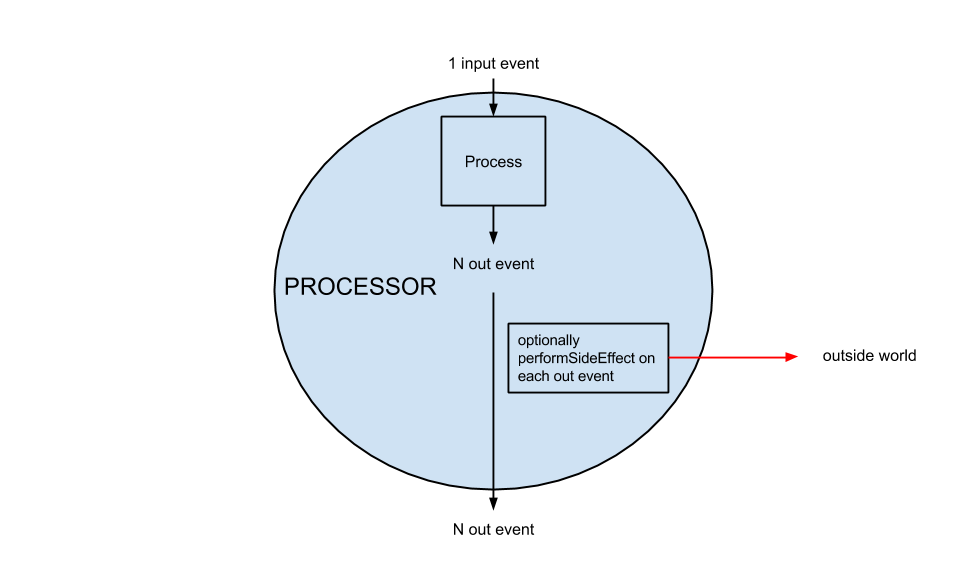
\includegraphics[width=1.0\textwidth]{img/stream_processor.png}}
    \caption{A stream processor}
    \label{fig:streamprocessor}
  \end{center}
\end{figure}

\begin{figure}[H]
  \begin{center} 
    \makebox[\textwidth]{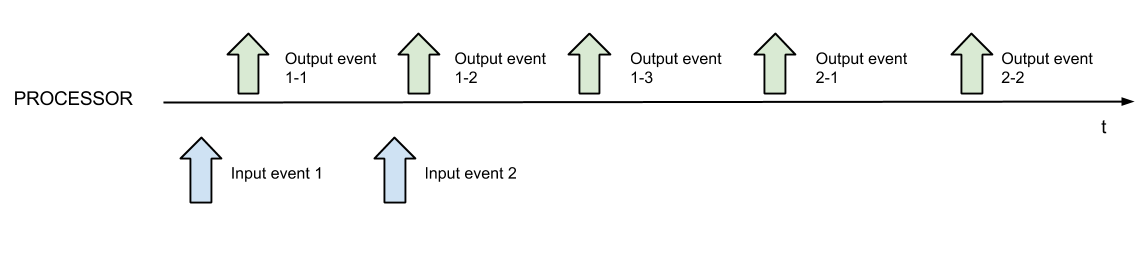
\includegraphics[width=1.0\textwidth]{img/substream.png}}
    \caption{In-order insertion of a sub-stream in a stream}
    \label{fig:substream}
  \end{center}
\end{figure}

Another important functional requirement for processors is that the \verb|process| and \verb|performSideEffect| methods can ensure the
sequentiality of asynchronous non-blocking operations (for example, a side-effect or a processing can be done via an asynchronous call to a 
database, but despite the asynchronous nature of the call the processor must wait that the asynchronous call has returned
before processing the next event). Even sub-stream production can be asynchronous, meaning that the production of a sub-stream
can be a composition of asynchronous operations (like pulling from a database with an asynchronous non-blocking driver).

Last but not least, the platform must ensure no message loss or duplication even in case of a temporary failure of a processor. This means that a processor
that had a transient failure must be able to \textit{replay} the stream from where it was before its crash.

\section{Non-functional requirements}

This section details the following non-functional requirements:
\begin{itemize}
  \item Easy scale up and scale out with a share-nothing architecture.
  \item Decoupled processors that can consume the stream with heterogeneous processing speeds without affecting each other.
  \item Optimized resource consumption in the whole system with non-blocking IO.
  \item All the previous non-functional requirements should ensure a soft real-time property (as defined in the introduction). In a few words, for a realistic event push rate as in the business use case application, the end-to-end event processing latency should be measured in seconds (not minutes or hours).
\end{itemize}

\subsection{Data Integration}

The Data Integration part must be able to scale up easily as one of the goals of the platform is to potentially handle high push rates of events. Scale up means that the puller should automatically make the best possible use of all cores available on a machine in order to parallelize the various pulls. The different parts of the puller should also be easily distributable in case of the load if too big for one machine to handle. 

To prevent software and/or hardware faults that can happen in every kind of IT systems, the puller should also be fault-tolerant, i.e if a component experiences a transient failure, the system should ensure that no event is duplicated or lost.

Moreover, the nature of the puller implies that it will spend the majority of its time doing IO to query different data sources.
Those IOs can have various durations depending on the size of the data to pull, the latency and bandwidth of the data sources, etc.
We want to optimize the use of resource (CPU, RAM) despite the fact that the platform is very IO-oriented. This enables to maximize the event push rate that a given machine can handle, and therefore minimize the cost of the infrastructure once the platform is in production. Chapter \ref{chap:study} will show how asynchronous non-blocking IO meets these expectations. 

Another non-functional requirement is to have clean and composable code source despite its asynchronous nature. Asynchronous
code can indeed lead to maintenance nightmare if the wrong abstractions are used. Chapter \ref{chap:study} will
show that the use of functional programming solves these problems.

\subsection{Journal and Stream Processing}

The Journal and Stream Processing part requires complex non-functional requirements in order to optimize resource consumption and maximize performance.

A common problem with stream processing is to manage the flow rate. A producer can indeed produce events at a rate superior to
the processing rate of a consumer. This problem is even more important when there is a tree-like structure of stream processors instead of a linear structure. Indeed, the platform should handle the fact that even if sibling processors in the tree have different processing speeds, they do not block each other based on the slowest sibling. In other words, sibling processors should be totally decoupled so that when a new event is sent from a parent to its children, the parent does not have to wait that its slowest
children has finished to process the event in order to send the next event to them. This property guarantees that a long processing will not slow down other parallel slow processing (so that an event stream that goes only through fast processors can keep a low latency). This problem should be handled while minimizing RAM consumption in order to make the best use of the resources in the system so that a given resource configuration can handle a higher push rate of events.

Stream processors should also be easily distributable in order to deal with event flows that are too big for one machine to handle.




\newpage
\printbibliography

\newpage
\listoffigures

\newpage
\appendix
\addappheadtotoc
\chapter{RDF}\label{appA}

\begin{figure}[ht]
\begin{center}
And here is a figure
\caption{\small{Several statements describing the same resource.}}\label{RDF_4}
\end{center}
\end{figure}

that we refer to here: \ref{RDF_4}
\end{document}
